% chapters/cap6_resultados/cap6.tex

\chapter{Resultados y Discusión}
\label{cap:resultados}

Este capítulo contrasta la relajación del dímero SPH~\eqref{eq:sph_advection_discrete} con el circuito abierto descrito en el capítulo~\ref{cap:implementacion_circuito}. En todos los ensayos cuánticos se emplearon $4000$ lanzamientos. Los parámetros físicos son los mismos que los puestos en el capítulo~\ref{cap:metodologia}.
\section{Referencia clásica y simulación cuántica}

La referencia clásica se construye con la ecuación de advección discreta~\eqref{eq:sph_advection_discrete}. Ese esquema es recursivo ya que el estado en $t_0+\Delta t$ exige conocer el estado en $t_0$. Cada incremento temporal reutiliza las cantidades $u_j(t_0)$ de ambas partículas, de forma que el detalle de la trayectoria depende de $\Delta t$, mientras se reduce este valor mejor es el detalle y por ende, el comportamiento se apega más a la realidad. El resultado se muestra en la figura~\ref{fig:cassical_sim}.

\begin{figure}[htbp]
    \centering
    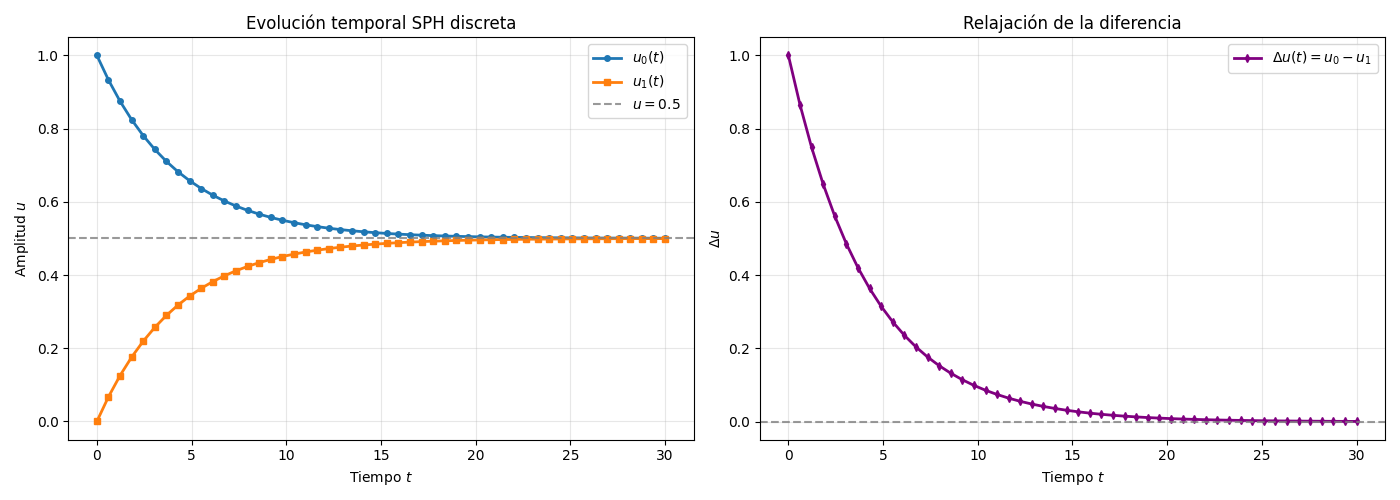
\includegraphics[width=0.95\textwidth]{chapters/cap6_resultados/img/clasical.png}
    \caption{Simulación clásica de dos partículas con la discretización SPH~\eqref{eq:sph_advection_discrete}.}
    \label{fig:cassical_sim}
\end{figure}

La simulación cuántica emplea el mismo escenario: dos partículas, la misma condición inicial y los mismos parámetros. El bloque elemental es el de la figura~\ref{fig:circ-medida-inter}, repetido $100$ veces. Las curvas cuánticas corresponden a las poblaciones $P_j = \rho_{jj}$, identificadas con $u_j$ como se indicó en la sección~\ref{sec:codificacion_estado}. Para reconstruir la curva se muestrearon $40$ instantes uniformes entre $t=0$ y $t=30$. El resultado aparece en la figura~\ref{fig:sim_definitive}. Ambas evoluciones son comparables: la cantidad advectada abandona la partícula $0$, se transfiere a la partícula $1$ y se aproxima al equilibrio en $0{,}5$, sin el rebote sinusoidal del circuito cerrado. Ese equilibrio es el de la ODE~\eqref{eq:sph_advection_discrete} con partículas fijas.

\begin{figure}[htbp]
    \centering
    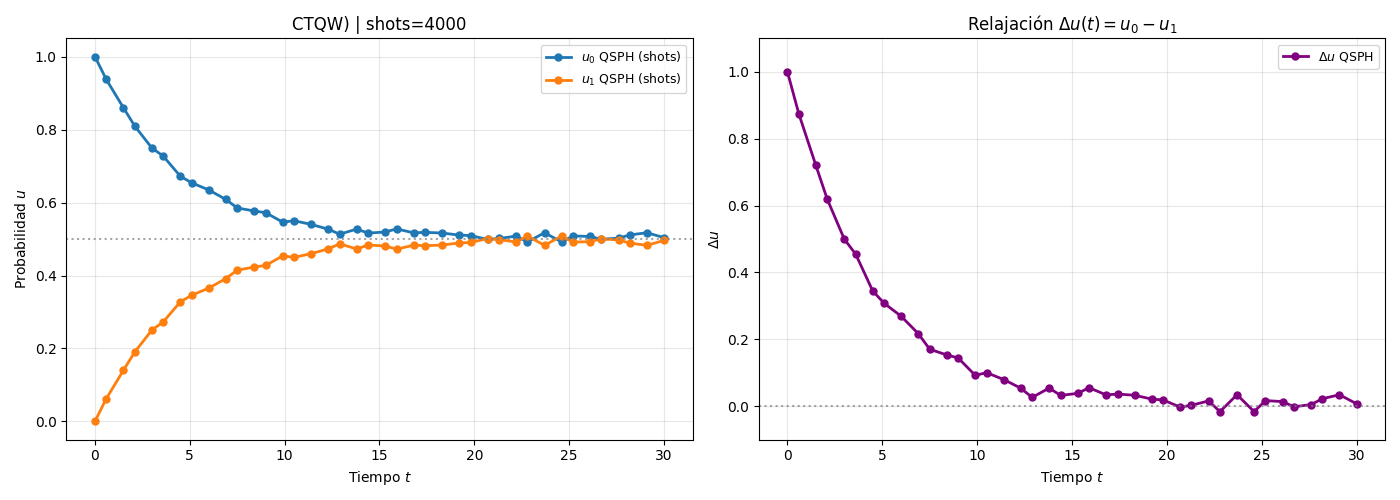
\includegraphics[width=0.95\textwidth]{chapters/cap6_resultados/img/cuantum-sim.png}
    \caption{Simulación cuántica con Hamiltoniano efectivo, ancilla y medición intermedia. Se muestran las poblaciones $P_j$, identificadas con $u_j$, y $40$ instantes para comparar el comportamiento con la referencia clásica.}
    \label{fig:sim_definitive}
\end{figure}

\section{Lectura del estado inicial y final}

La figura~\ref{fig:sim_definitive} sirve para comparar trayectorias. No es, sin embargo, un requisito del algoritmo cuántico. El esquema clásico no puede saltar de $t=0$ a $t=30$ sin calcular los estados intermedios. En cambio el algoritmo cuántico sí, basta concatenar los $100$ bloques de la figura~\ref{fig:circ-medida-inter} y medir el qubit del sistema al final. La figura~\ref{fig:ventaja} muestra únicamente esos dos extremos. El estado inicial y el estado a $t=30$ coinciden con los de la curva completa, sin recorrer el camino punto a punto.

\begin{figure}[htbp]
    \centering
    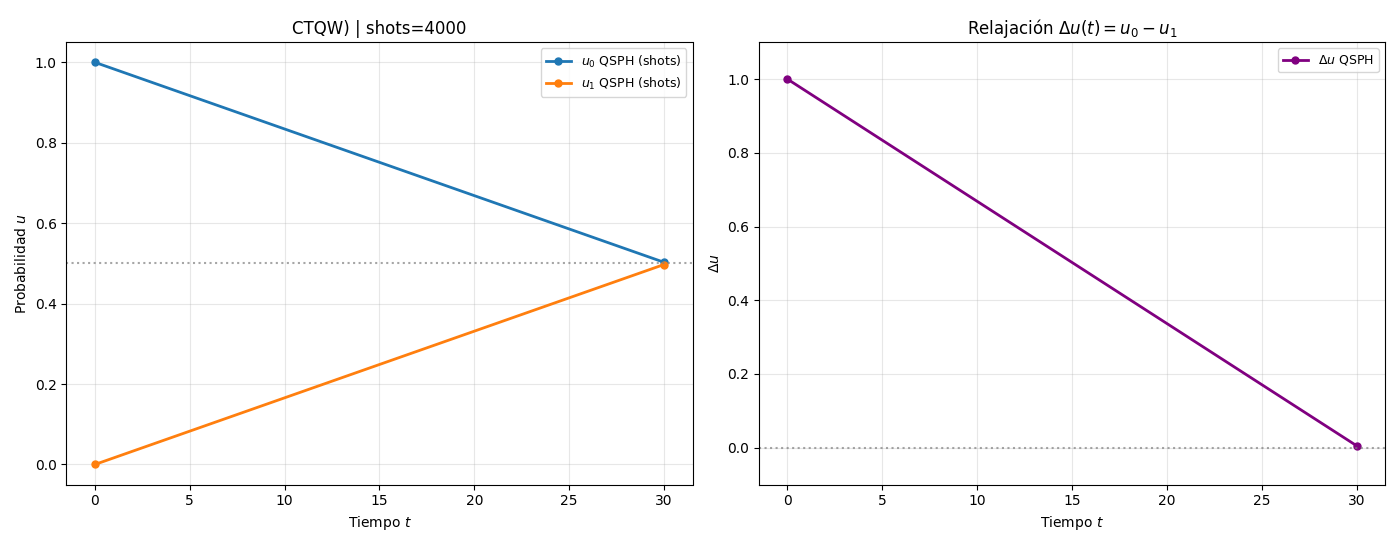
\includegraphics[width=0.95\textwidth]{chapters/cap6_resultados/img/ventaja.png}
    \caption{Lectura directa del estado inicial y del estado a $t=30$ tras aplicar $100$ bloques de Trotter, sin reconstruir la trayectoria intermedia.}
    \label{fig:ventaja}
\end{figure}

\begin{figure}[htbp]
    \centering
    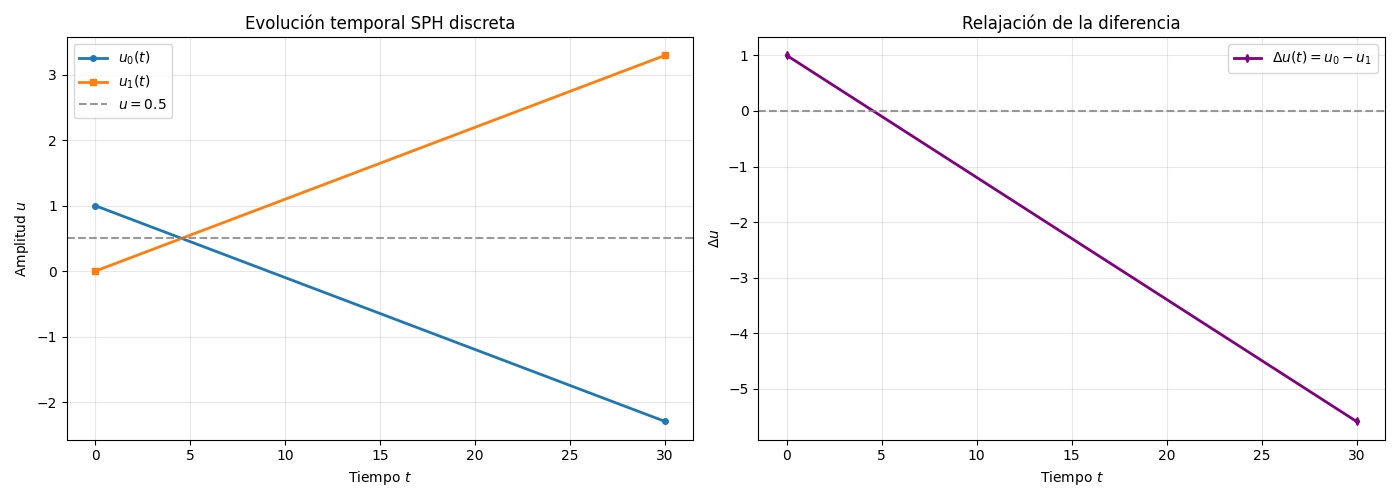
\includegraphics[width=0.95\textwidth]{chapters/cap6_resultados/img/classic-0-a-30-un-paso.png}
    \caption{Lectura directa del estado inicial y del estado a $t=30$ con simulación clásica}
    \label{fig:ventaja_classic}
\end{figure}

Esta diferencia es operativa. La gráfica de $40$ puntos se usó solo para validar el comportamiento. Una vez aceptada la correspondencia con la ecuación (\eqref{eq:sph_advection_discrete}), el circuito puede ejecutarse de una vez sobre el intervalo completo y devolver la cantidad advectada final. Es una diferencia de este circuito de Trotter concatenado frente al Euler recursivo en $N=2$, no una demostración de \emph{speedup} asintótico.

\section{Variación de la velocidad de advección}

Como comprobación adicional se realizarón más pruebas variando la velocidad de advección $c$ de $10^{-0{,}5}$ a $10^{-1}$ y $10^{-0.2}$, manteniendo el resto de parámetros. Disminuir $c$ debilita el acoplamiento entre partículas, en la misma dirección que los ensayos de ~\cite{auyeung2025}, donde una menor interacción retrasa el transporte de la cantidad advectada. Las figuras~\ref{fig:clasico-c-menor} y~\ref{fig:cuantico-c-menor} muestran el caso clásico y el cuántico. A $t=30$ el sistema ya no alcanza el equilibrio en $0{,}5$: la transferencia es más lenta y ambas descripciones vuelven a coincidir. 

Por otro lado el hecho de aumentar $c$ aumenta la fuerza de acoplamiento haciendo que la interacción y relajación suceda de forma más rápida, tal como se ve en \ref{fig:clasico-c-mayor} y en \ref{fig:cuantico-c-mayor}. El circuito sigue, por tanto, la relajación de la ecuación~\eqref{eq:sph_advection_discrete} al variar $c$.

\begin{figure}[htbp]
    \centering
    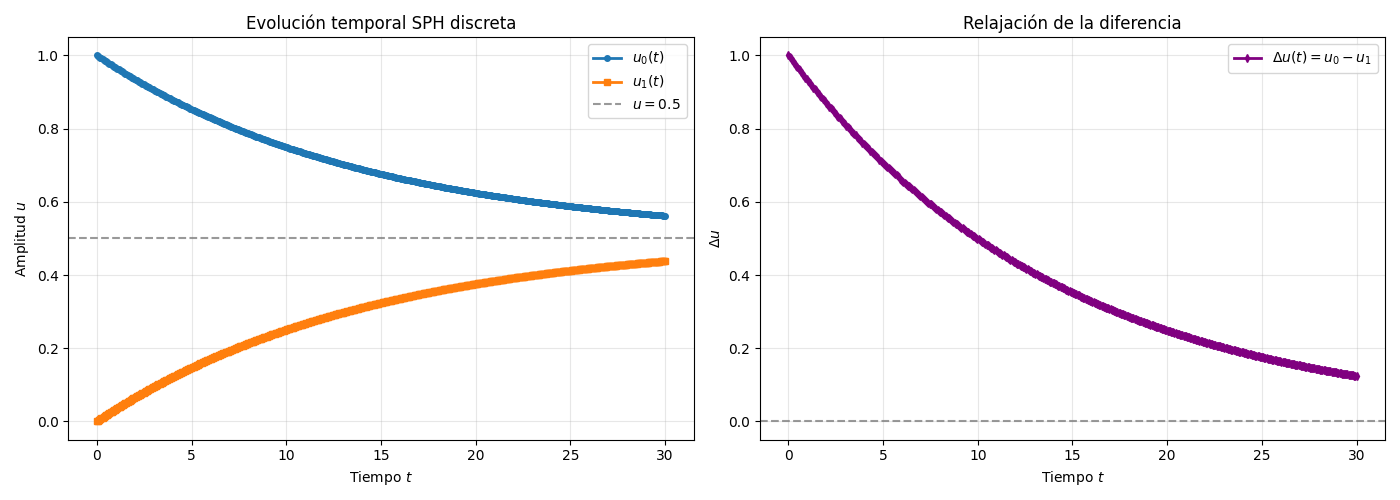
\includegraphics[width=0.95\textwidth]{chapters/cap6_resultados/img/cla-c-menor.png}
    \caption{Simulación clásica con $c=10^{-1}$.}
    \label{fig:clasico-c-menor}
\end{figure}

\begin{figure}[htbp]
    \centering
    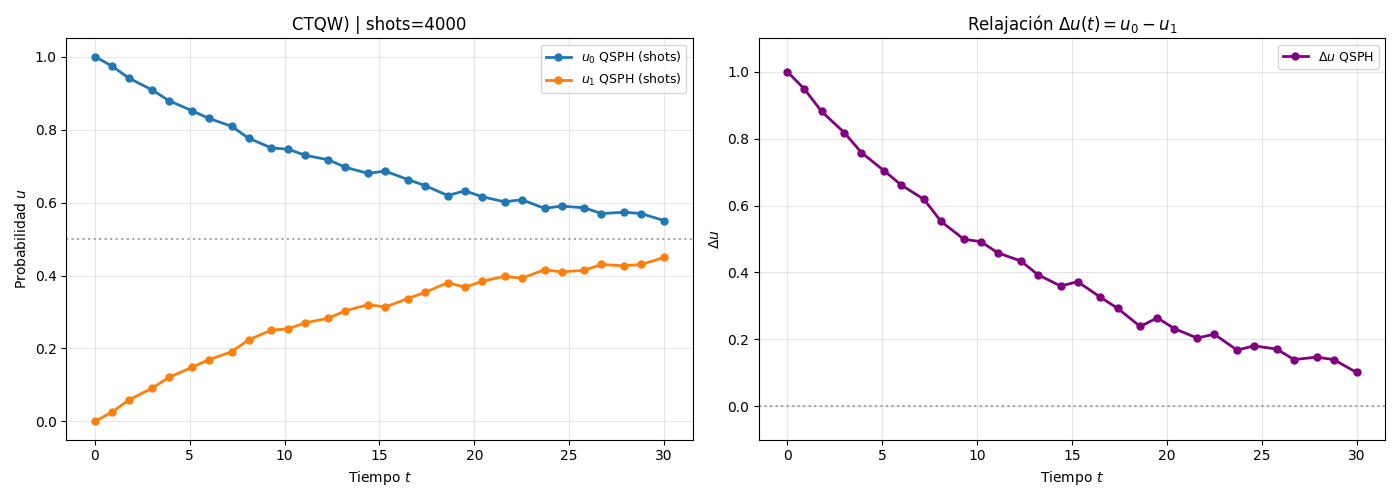
\includegraphics[width=0.95\textwidth]{chapters/cap6_resultados/img/cua-c-menor.png}
    \caption{Simulación cuántica con $c=10^{-1}$.}
    \label{fig:cuantico-c-menor}
\end{figure}

\begin{figure}[htbp]
    \centering
    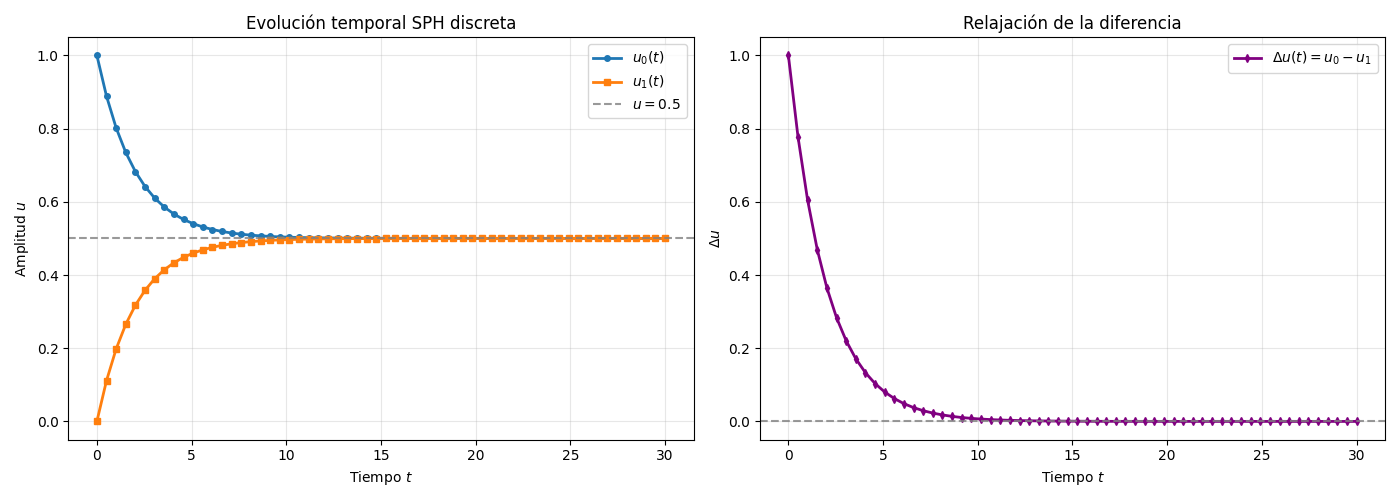
\includegraphics[width=0.95\textwidth]{chapters/cap6_resultados/img/cla-c-mayor.png}
    \caption{Simulación cuántica con $c=10^{-0.2}$.}
    \label{fig:cuantico-c-mayor}
\end{figure}

\begin{figure}[htbp]
    \centering
    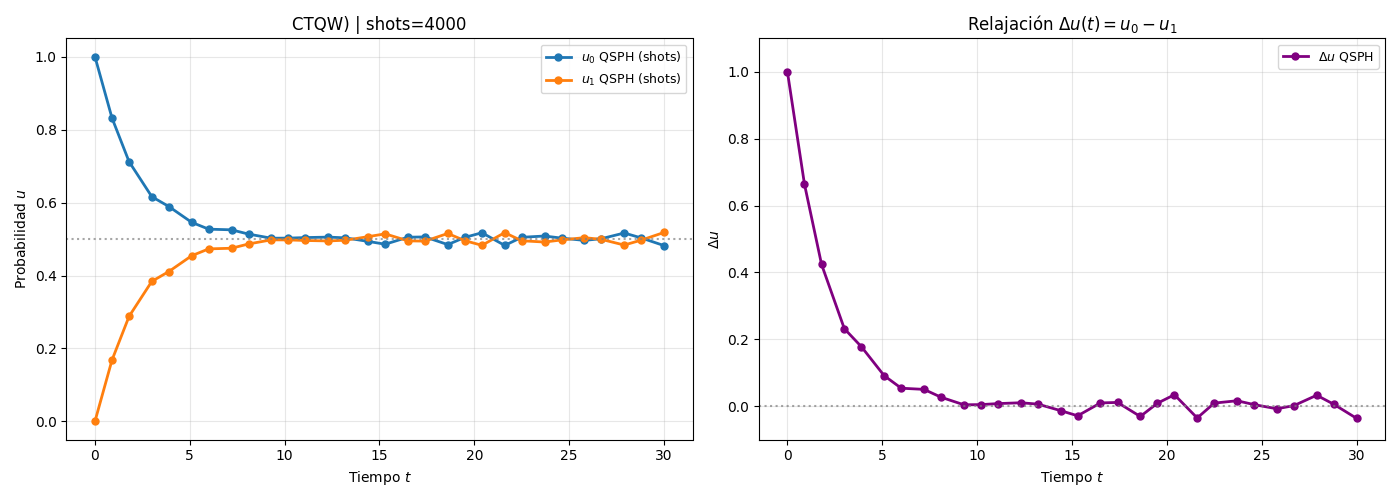
\includegraphics[width=0.95\textwidth]{chapters/cap6_resultados/img/cua-c-mayor.png}
    \caption{Simulación cuántica con $c=10^{-0.2}$.}
    \label{fig:clasico-c-mayor}
\end{figure}
